\documentclass[12pt]{article}

\usepackage[utf8]{inputenc}
\usepackage[a4paper]{geometry}

% math packages
\usepackage{amssymb, amsmath, amsbsy, amsthm, amsfonts, amscd}
\usepackage{enumerate}
\usepackage{array}
\usepackage{booktabs}
\usepackage{graphicx}
\usepackage{float}
\usepackage{xcolor}
\usepackage[colorlinks=true,linkcolor=blue!50!black,citecolor=blue!50!black,urlcolor=blue!50!black]{hyperref}

% formatting & headers
\usepackage{fancyhdr}
\setlength{\headheight}{15pt}
\usepackage{lastpage}

\pagestyle{fancy}
\fancyhf{}
\lhead{MAT386H5 -- Fall 2026}
\chead{}
\rhead{VIX$^2$ Derivation and VIX Computation}
\cfoot{\thepage\ of \pageref{LastPage}}

\newcommand{\E}{\mathbb{E}^{\mathbb{Q}}}
\newcommand{\Kvar}{K_{\mathrm{var}}}
\newcommand{\VIX}{\mathrm{VIX}}

% end of setup

\begin{document}

\begin{center}
  {\Large\bfseries VIX$^2$ as the Fair Strike of a Variance Swap,\\[2pt] and Computing the VIX from S\&P~500 Options}\\[6pt]
  MAT386 Group Project --- Pricing/hedging (Section~1) and Simulation (Section~1)
\end{center}

\noindent This part derives VIX$^2$ as the fair strike of a 30-day variance swap by static replication with out-of-the-money options, and then implements the Cboe formula on real option quotes. Our implementation reproduces Cboe's published worked example to eight decimal places and, on a live snapshot taken on 5 November 2026, gives a VIX of 22.49 against the official 22.54.

%=====================================================================
\section{VIX$^2$ as the fair strike of a variance swap}
%=====================================================================

\subsection{Setup}

We work under the risk-neutral measure $\mathbb{Q}$ with a constant interest rate $r$ and dividend yield $q$. The S\&P~500 index $S_t$ follows a diffusion whose volatility $\sigma_t$ may itself be random, so the result holds for the Heston model and any other stochastic-volatility model without jumps:
\begin{equation}
  \frac{dS_t}{S_t} = (r-q)\,dt + \sigma_t\,dW_t .
\end{equation}
The forward price for delivery at $T$ is $F_t = S_t e^{(r-q)(T-t)}$. It has no drift under $\mathbb{Q}$, and $F_T = S_T$:
\begin{equation}
  \frac{dF_t}{F_t} = \sigma_t\,dW_t .
  \label{eq:fwd}
\end{equation}
A variance swap with maturity $T$ pays, per unit of notional, the realised variance minus a strike $\Kvar$ agreed today. It costs nothing to enter, so the fair strike is the risk-neutral expectation of realised variance:
\begin{equation}
  \text{Payoff} = \frac{1}{T}\int_0^T \sigma_t^2\,dt - \Kvar,
  \qquad
  \Kvar = \E\!\left[\frac{1}{T}\int_0^T \sigma_t^2\,dt\right].
\end{equation}
We show that $\Kvar$ can be written using only today's prices of out-of-the-money options, $Q(K)$, which is a put $P(K)$ for $K<K_0$ and a call $C(K)$ for $K>K_0$:
\begin{equation}
  \Kvar = \frac{2e^{rT}}{T}\int_0^{\infty}\frac{Q(K)}{K^2}\,dK
  \;-\; \frac{2}{T}\left[\frac{F_0}{K_0}-1-\ln\frac{F_0}{K_0}\right]
  \label{eq:result}
\end{equation}
The VIX is the discrete version of \eqref{eq:result} with $T=30$ days, and $\VIX = 100\sqrt{\Kvar}$.

\subsection{Step 1: variance is a log contract}

Apply It\^o's lemma to $g(F)=\ln F$, with $g'(F)=1/F$, $g''(F)=-1/F^2$ and $(dF_t)^2=\sigma_t^2F_t^2\,dt$ from \eqref{eq:fwd}:
\begin{equation}
  d\ln F_t = \frac{dF_t}{F_t} - \frac{1}{2}\frac{(dF_t)^2}{F_t^2}
           = \frac{dF_t}{F_t} - \frac{1}{2}\sigma_t^2\,dt .
\end{equation}
Integrating from $0$ to $T$ and using $F_T=S_T$,
\begin{equation}
  \int_0^T \sigma_t^2\,dt = 2\int_0^T \frac{dF_t}{F_t} \;-\; 2\ln\frac{S_T}{F_0}.
  \label{eq:decomp}
\end{equation}
The stochastic integral $\int_0^T dF_t/F_t=\int_0^T\sigma_t\,dW_t$ has zero expectation under $\mathbb{Q}$, so
\begin{equation}
  \Kvar = -\frac{2}{T}\,\E\!\left[\ln\frac{S_T}{F_0}\right].
  \label{eq:logcontract}
\end{equation}
Pricing a variance swap is therefore equivalent to pricing a \emph{log contract}, a claim paying $\ln(S_T/F_0)$ at $T$. The path of $\sigma_t$ has dropped out.

\subsection{Step 2: replicating the log contract with options}

Any twice-differentiable payoff $f(S_T)$ can be built from a bond, a forward and a strip of out-of-the-money options \cite{carrmadan}. For any reference strike $K_0$,
\begin{equation}
\begin{split}
  f(S_T) = f(K_0) &+ f'(K_0)(S_T-K_0)\\
  &+ \int_0^{K_0} f''(K)\,(K-S_T)^+\,dK
  + \int_{K_0}^{\infty} f''(K)\,(S_T-K)^+\,dK .
\end{split}
  \label{eq:carrmadan}
\end{equation}
\textit{Proof.} Taylor's theorem with integral remainder gives
$f(S) = f(K_0) + f'(K_0)(S-K_0) + \int_{K_0}^{S} f''(K)(S-K)\,dK$.
If $S>K_0$ the remainder equals $\int_{K_0}^{\infty} f''(K)(S-K)^+\,dK$, because $(S-K)^+=0$ for $K\ge S$, and the put integral in \eqref{eq:carrmadan} is zero. If $S<K_0$ the remainder equals $\int_{S}^{K_0} f''(K)(K-S)\,dK=\int_0^{K_0} f''(K)(K-S)^+\,dK$, and the call integral is zero. Hence \eqref{eq:carrmadan} holds for every $S$. \hfill$\square$

For $f(S)=\ln S$ we have $f'(K_0)=1/K_0$ and $f''(K)=-1/K^2$. Subtracting $\ln F_0$ from both sides,
\begin{equation}
  \ln\frac{S_T}{F_0} = \ln\frac{K_0}{F_0} + \frac{S_T-K_0}{K_0}
  - \int_0^{K_0}\frac{(K-S_T)^+}{K^2}\,dK
  - \int_{K_0}^{\infty}\frac{(S_T-K)^+}{K^2}\,dK .
  \label{eq:logrep}
\end{equation}
The log payoff is a constant, plus $1/K_0$ forwards, minus puts below $K_0$ and calls above $K_0$ held in quantity $1/K^2$ per unit of strike. The $1/K^2$ weights are the second derivative of the logarithm.

\subsection{Step 3: pricing the replication}

Under $\mathbb{Q}$, $\E[S_T]=F_0$ and each option's expected payoff is its price grown at the risk-free rate, $\E[(K-S_T)^+]=e^{rT}P(K)$ and $\E[(S_T-K)^+]=e^{rT}C(K)$. Taking expectations of \eqref{eq:logrep},
\begin{equation}
  \E\!\left[\ln\frac{S_T}{F_0}\right] = \ln\frac{K_0}{F_0} + \frac{F_0-K_0}{K_0}
  - e^{rT}\int_0^{\infty}\frac{Q(K)}{K^2}\,dK .
\end{equation}
Substituting into \eqref{eq:logcontract} and using $\ln(K_0/F_0)=-\ln(F_0/K_0)$ gives \eqref{eq:result}. The result is exact under the assumptions above, and every quantity on the right-hand side is observable today: no volatility model enters.

\subsection{Step 4: from the integral to the Cboe formula}

Three approximations turn \eqref{eq:result} into the formula Cboe publishes \cite{cboewp,cboemeth}.

\begin{enumerate}
  \item \textbf{Correction term.} Let $x=F_0/K_0-1$. Since $K_0$ is the listed strike just below $F_0$, $x$ is small ($x\approx 0.0015$ in Cboe's example). Using $\ln(1+x)=x-\tfrac{1}{2}x^2+O(x^3)$,
  \begin{equation}
    \frac{2}{T}\bigl[x-\ln(1+x)\bigr] = \frac{1}{T}\left(\frac{F_0}{K_0}-1\right)^2 + O\!\left(\frac{x^3}{T}\right),
  \end{equation}
  where the neglected term is of order $10^{-9}$ in the example.
  \item \textbf{Discrete strikes.} Options trade at listed strikes $K_i$, so the integral becomes a sum with $\Delta K_i=\tfrac{1}{2}(K_{i+1}-K_{i-1})$ (the gap to the single neighbour at the ends). The interval of $K_0$ lies half in the put region and half in the call region, which is why Cboe uses $Q(K_0)=\tfrac{1}{2}\bigl(P(K_0)+C(K_0)\bigr)$. The strip stops after two consecutive zero bids.
  \item \textbf{Constant 30-day maturity.} Cboe computes $\sigma^2$ for the two expirations that bracket 30 days and interpolates linearly in total variance $T\sigma^2$.
\end{enumerate}
The result is, for each expiration,
\begin{equation}
  \sigma^2 = \frac{2}{T}\sum_i \frac{\Delta K_i}{K_i^2}\,e^{RT}Q(K_i) - \frac{1}{T}\left(\frac{F}{K_0}-1\right)^2,
  \qquad F = K^* + e^{RT}\bigl(C(K^*)-P(K^*)\bigr),
  \label{eq:cboe}
\end{equation}
where $K^*$ is the strike minimising $|C(K)-P(K)|$, and
\begin{equation}
  \VIX = 100\sqrt{\left\{T_1\sigma_1^2\frac{N_{T_2}-N_{30}}{N_{T_2}-N_{T_1}} + T_2\sigma_2^2\frac{N_{30}-N_{T_1}}{N_{T_2}-N_{T_1}}\right\}\frac{N_{365}}{N_{30}}},
  \label{eq:interp}
\end{equation}
with $N$ denoting times in minutes. Table~\ref{tab:map} maps each term to Cboe's worked example.

\begin{table}[H]
\centering
\small
\begin{tabular}{@{}lll@{}}
\toprule
\textbf{Derivation} & \textbf{Cboe formula} & \textbf{Cboe example}\\
\midrule
Option strip $\frac{2e^{rT}}{T}\int Q(K)K^{-2}dK$ & $\frac{2}{T}\sum_i \frac{\Delta K_i}{K_i^2}e^{RT}Q(K_i)$ & 0.018495\\[3pt]
Correction $\frac{2}{T}[x-\ln(1+x)]$ & $\frac{1}{T}(F/K_0-1)^2$ & 0.00003203\\[3pt]
$\Kvar$ for one expiry & $\sigma_1^2$ & 0.01846292\\[3pt]
$\sqrt{\Kvar}$ at 30 days & $\VIX/100$ & 0.13685821\\
\bottomrule
\end{tabular}
\caption{Terms of the derivation and their counterparts in the Cboe formula, with the values from Cboe's worked example \cite{cboewp}.}
\label{tab:map}
\end{table}

\subsection{Interpretation}

\paragraph{The replicating hedge.} By \eqref{eq:decomp},
\begin{equation}
  \frac{1}{T}\int_0^T\sigma_t^2\,dt
  = \underbrace{-\frac{2}{T}\ln\frac{S_T}{F_0}}_{\text{static option strip}}
  \;+\; \underbrace{\frac{2}{T}\int_0^T\frac{dF_t}{F_t}}_{\text{dynamic futures position}} .
\end{equation}
A dealer who sells a variance swap buys the strip of out-of-the-money options in quantity $2/(TK^2)$ per unit of strike and holds $2/(TF_t)$ futures, rebalanced as $F_t$ moves. Futures cost nothing to enter, so the fair strike equals the cost of the option strip. The strip itself is never rebalanced, hence \emph{static} replication \cite{ddkz}.

\paragraph{Why $1/K^2$.} An option earns from volatility through its gamma; its dollar gamma $\tfrac{1}{2}S^2\Gamma$ is concentrated near its strike and scales roughly with $K^2$. Weighting each option by $1/K^2$ makes the strip's total dollar gamma the same at every index level, so the portfolio is exposed to variance alone and not to the level of the index \cite{ddkz}.

\paragraph{Model-free.} The derivation allowed $\sigma_t$ to follow any path, so the VIX reads the market's expected variance directly from option prices without a pricing model, unlike Black--Scholes implied volatility. Because low strikes receive the largest weights and are the most expensive under the volatility skew, out-of-the-money puts dominate the index (Section~\ref{sec:live}).

\paragraph{Link to VIX futures.} The replication prices VIX$^2$, not VIX. Since the square root is concave, Jensen's inequality gives $\E[\VIX_T]\le\sqrt{\E[\VIX_T^2]}$: a VIX future is worth less than the square root of the forward variance strike. This gap is the convexity adjustment measured in the Heston section.

\subsection{Assumptions and where they break}

\begin{table}[H]
\centering
\small
\begin{tabular}{@{}p{3.7cm}p{4.5cm}p{5.4cm}@{}}
\toprule
\textbf{Assumption} & \textbf{In practice} & \textbf{Effect}\\
\midrule
Continuous paths (no jumps) & The index can gap (e.g.\ 5 Feb 2018) & VIX$^2$ differs from the variance-swap strike by a term in the cube of the jump sizes \cite{carrwu}\\
Continuum of strikes on $(0,\infty)$ & Listed strikes come in steps & Small discretisation error\\
Every strike has a price & Strip stops after two zero bids & Truncation lowers the VIX slightly, more in stressed markets\\
Constant $r$ and $q$ & Rates change over 30 days & Negligible at a 30-day horizon\\
Second-order expansion & Exact term is $x-\ln(1+x)$ & Error of order $x^3$\\
Linear interpolation in $T\sigma^2$ & Term structure can curve & Small; both expiries are within a week of 30 days\\
\bottomrule
\end{tabular}
\caption{Assumptions behind \eqref{eq:result} and the effect of relaxing them. The middle four are built into the official index itself.}
\label{tab:assumptions}
\end{table}

%=====================================================================
\section{Computing the VIX from option quotes}
%=====================================================================

\subsection{Data}

We took a snapshot of S\&P~500 index options from Yahoo Finance (15-minute delayed quotes) on \textbf{5 November 2026 at 11:41 ET}, together with the S\&P~500 level (7,476.22) and the official VIX at the same moment (22.54). The snapshot contains 2,118 SPXW options across ten expirations between 27 November and 11 December 2026; 97.8\% have a positive bid. Risk-free rates are the 1- and 3-month constant-maturity Treasury yields from the US Treasury daily par yield curve (4.01\% and 4.21\% on 4 November 2026).

\subsection{Implementation}

The calculation (\texttt{vix\_calc.py}) follows the Cboe methodology \cite{cboemeth}:
\begin{enumerate}
  \item \textbf{Expirations.} Select the first two Friday expirations more than 23 and fewer than 37 days away. Standard third-Friday SPX options settle at 9:30 ET; weekly SPXW options settle at 16:00 ET. Time to expiry is measured in minutes, $T=M/525{,}600$.
  \item \textbf{Rates.} Interpolate the 1-month (30-day) and 3-month (91-day) Treasury yields linearly to each expiry, then convert each from a bond-equivalent yield (BEY) to a continuously compounded rate, as Cboe does:
  \[ \mathrm{APY}=\left(1+\tfrac{\mathrm{BEY}}{2}\right)^2-1, \qquad R=\ln(1+\mathrm{APY}). \]
  \item \textbf{Forward and $K_0$.} Use mid-quotes; find $K^*$ minimising $|C-P|$, compute $F$ from \eqref{eq:cboe}, and take $K_0$ as the first strike at or below $F$.
  \item \textbf{Strike selection.} Out-of-the-money puts below $K_0$ and calls above $K_0$, skipping zero bids and stopping after two consecutive zero bids; the average of put and call at $K_0$.
  \item \textbf{Variance and interpolation.} Apply \eqref{eq:cboe} to each expiry and \eqref{eq:interp} to obtain the 30-day VIX.
\end{enumerate}

\subsection{Validation against Cboe's worked example}

Before using live data, we ran the same code on the option data in Appendix~1 of the Cboe VIX White Paper \cite{cboewp} (186 near-term and 128 next-term strikes, extracted from the PDF text), with Cboe's stated inputs ($T$ in minutes, $R_1=0.0305\%$, $R_2=0.0286\%$). Table~\ref{tab:cboe} shows that every intermediate quantity matches.

\begin{table}[H]
\centering
\small
\begin{tabular}{@{}lrr@{}}
\toprule
\textbf{Quantity} & \textbf{Our code} & \textbf{Cboe}\\
\midrule
$T_1$ & 0.06834855 & 0.0683486\\
$T_2$ & 0.08826865 & 0.0882686\\
$F_1$ & 1962.89996 & 1962.89996\\
$F_2$ & 1962.40006 & 1962.40006\\
$K_0$ (both terms) & 1960 & 1960\\
$\sigma_1^2$ & 0.01846292 & 0.01846292\\
$\sigma_2^2$ & 0.01882101 & 0.01882101\\
VIX & 13.685821 & 13.685821\\
\bottomrule
\end{tabular}
\caption{Our implementation on Cboe's worked example. The only differences are in $T$, where Cboe rounds to seven decimals. Because $\sigma^2$ depends on every selected strike, the match also confirms that the code selects exactly the same strikes as Cboe.}
\label{tab:cboe}
\end{table}

\subsection{Live result: 5 November 2026}
\label{sec:live}

\begin{table}[H]
\centering
\small
\begin{tabular}{@{}lrr@{}}
\toprule
 & \textbf{Near term} & \textbf{Next term}\\
\midrule
Expiry (SPXW, 16:00 ET) & Fri 4 Dec 2026 & Fri 11 Dec 2026\\
Minutes to settlement & 42,018 (29.18 days) & 52,098 (36.18 days)\\
$T$ (years) & 0.079944 & 0.099122\\
$R$ (continuous) & 0.039703 & 0.039902\\
$K^*$ & 7,500 & 7,500\\
Forward $F$ & 7,498.0438 & 7,501.4055\\
$K_0$ & 7,490 & 7,500\\
Strikes used (puts / $K_0$ / calls) & 89 / 1 / 87 & 51 / 1 / 54\\
Strike range & 3,200--8,700 & 3,200--9,000\\
$\sigma^2$ (volatility) & 0.050506 (22.47\%) & 0.050951 (22.57\%)\\
30-day weight & 0.8828 & 0.1172\\
\midrule
\textbf{Calculated VIX} & \multicolumn{2}{r}{\textbf{22.49}}\\
\textbf{Official VIX} & \multicolumn{2}{r}{\textbf{22.54}}\\
\textbf{Difference} & \multicolumn{2}{r}{$-0.05$ points}\\
\bottomrule
\end{tabular}
\caption{VIX computed from the 5 November 2026 snapshot.}
\label{tab:live}
\end{table}

The calculated VIX is within 0.05 points (0.2\%) of the official value. The remaining gap comes from inputs rather than the formula: Cboe interpolates rates with a cubic spline across the whole Treasury curve while we use two points; the option quotes and the official value were recorded seconds apart and are delayed; and Cboe's real-time quote feed and filtering differ from Yahoo's quotes.

A VIX of 22.5 means the market expects S\&P~500 volatility of about 22.5\% a year, or roughly $\pm 22.5/\sqrt{12}\approx\pm6.5\%$ over the next 30 days. The previous day the VIX closed at 16.61 with the S\&P~500 at 7,688.62; by the snapshot the index had fallen 2.8\% and the VIX had risen by 5.9 points, the ``fear gauge'' behaviour described in the discussion section.

\begin{figure}[H]
  \centering
  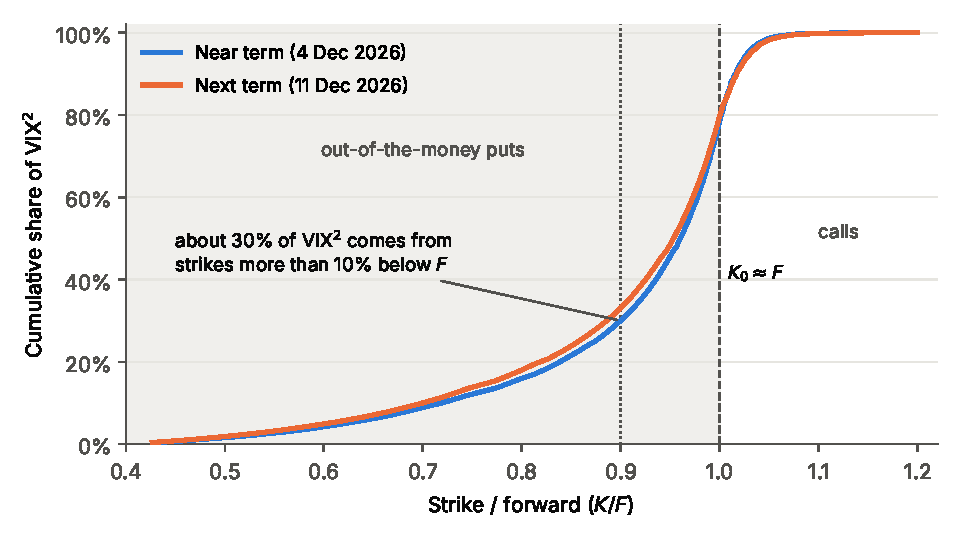
\includegraphics[width=0.85\linewidth]{figures/vix_strike_contributions.pdf}
  \caption{Cumulative share of $\sigma^2$ by strike, 5 November 2026 snapshot. About 76\% of the variance comes from out-of-the-money puts and 21\% from calls; roughly 30\% comes from puts more than 10\% below the forward.}
  \label{fig:contrib}
\end{figure}

Figure~\ref{fig:contrib} shows how the variance is built up across strikes. Puts supply about three quarters of VIX$^2$, and nearly a third comes from strikes more than 10\% below the forward. This is the combined effect of the $1/K^2$ weights and the skew: deep out-of-the-money puts are expensive because investors pay for crash protection. The VIX is therefore largely a price of crash insurance, which is why it rises sharply when the market falls.

\subsection{Numerical verification of the replication}

To confirm \eqref{eq:result} independently of Cboe's data, \texttt{verify\_variance\_replication.py} applies \eqref{eq:cboe} to option prices from two models in which the expected variance is known exactly. All prices use a forward of 100, $T=30/365$ and $r=4\%$.

\begin{table}[H]
\centering
\small
\begin{tabular}{@{}lrr@{}}
\toprule
\textbf{Strike grid} & \textbf{Strip variance} & \textbf{Volatility}\\
\midrule
Fine and wide (step 0.05, 20--300) & 0.040001 & 20.000\%\\
SPX-like spacing and range (step 0.07, 43--120) & 0.039997 & 19.999\%\\
Narrow range only (90--110) & 0.039056 & 19.763\%\\
Very coarse spacing only (step 5) & 0.045066 & 21.229\%\\
\bottomrule
\end{tabular}
\caption{Black--Scholes with $\sigma=20\%$ (true variance 0.04). The strip recovers the true variance; truncating the strike range lowers it and very coarse spacing raises it, as in Table~\ref{tab:assumptions}. A step of 0.07 at a forward of 100 matches SPX's 5-point spacing at 7,500.}
\label{tab:bs}
\end{table}

\begin{table}[H]
\centering
\small
\begin{tabular}{@{}lrr@{}}
\toprule
\textbf{Heston model, 200{,}000 Monte Carlo paths} & \textbf{Variance} & \textbf{Volatility}\\
\midrule
Exact expected variance $\theta+(v_0-\theta)\frac{1-e^{-\kappa T}}{\kappa T}$ & 0.028010 & 16.736\%\\
Simulated average realised variance & 0.028025 & 16.741\%\\
Option strip with $1/K^2$ weights & 0.028025 & 16.741\%\\
\bottomrule
\end{tabular}
\caption{Under Heston (parameters from \cite{gatheral}: $\kappa=1.3253$, $\theta=0.0354$, $\sigma=0.3877$, $\rho=-0.7165$, $v_0=0.0276$; full-truncation Euler, 24 steps per day), option prices are Monte Carlo averages over the same paths. The strip is within 0.1 standard errors of the exact value although volatility is random.}
\label{tab:heston}
\end{table}

Together, Tables~\ref{tab:cboe}--\ref{tab:heston} show that the formula is implemented correctly, that it reproduces the official index on live data, and that it recovers expected variance in a stochastic-volatility model, as the derivation predicts.

%=====================================================================
\appendix
\section{Data and code}
%=====================================================================

\begin{table}[H]
\centering
\small
\footnotesize
\begin{tabular}{@{}p{6.0cm}p{4.8cm}p{2.8cm}@{}}
\toprule
\textbf{File} & \textbf{Contents} & \textbf{Source}\\
\midrule
\texttt{data/options/}\newline\texttt{spx\_options\_20261105\_1141.csv} & SPX/SPXW options 20--40 days out, with spot and official VIX & Yahoo Finance\\
\texttt{data/risk\_free.csv} & Daily 1- and 3-month Treasury yields, 2010--2026 & US Treasury\\
\texttt{data/market\_history.csv} & Daily VIX, S\&P~500 and SPY (dividend-adjusted), 2010--2026 & Yahoo Finance\\
\texttt{data/vix\_futures\_all.csv} & Daily settlements of every monthly VX contract, Jan 2015--Feb 2027 & Cboe Futures Exchange\\
\texttt{data/vix\_front\_month.csv} & Front-month series rolled 5 trading days before expiry (used in the backtest) & Built from the above\\
\texttt{references/}\newline\texttt{cboe\_example\_*.csv} & Option data of Cboe's worked example & Cboe White Paper, App.~1\\
\midrule
\texttt{vix\_calc.py} & Computes the VIX from a snapshot & \\
\texttt{check\_cboe\_example.py} & Reproduces Table~\ref{tab:cboe} & \\
\texttt{verify\_variance\_replication.py} & Reproduces Tables~\ref{tab:bs}--\ref{tab:heston} & \\
\texttt{report/make\_vix\_figures.py} & Draws Figure~\ref{fig:contrib} & \\
\bottomrule
\end{tabular}
\end{table}

%=====================================================================
\begin{thebibliography}{9}
\bibitem{carrmadan} P.~Carr and D.~Madan (1998). Towards a theory of volatility trading. In R.~Jarrow (ed.), \emph{Volatility: New Estimation Techniques for Pricing Derivatives}, Risk Books.
\bibitem{ddkz} K.~Demeterfi, E.~Derman, M.~Kamal and J.~Zou (1999). \emph{More than you ever wanted to know about volatility swaps}. Goldman Sachs Quantitative Strategies Research Notes.
\bibitem{carrwu} P.~Carr and L.~Wu (2009). Variance risk premiums. \emph{Review of Financial Studies}, 22(3).
\bibitem{cboewp} Cboe (2019). \emph{Cboe Volatility Index White Paper}. \url{https://www.asx.com.au/content/dam/asx/investors/investment-options/vix/cboe-vix-white-paper.pdf}
\bibitem{cboemeth} Cboe Global Indices. \emph{Cboe Volatility Index Mathematics Methodology}.
\bibitem{hull} J.~C.~Hull (2022). \emph{Options, Futures, and Other Derivatives}, 11th ed. Pearson.
\bibitem{shreve} S.~E.~Shreve (2004). \emph{Stochastic Calculus for Finance II: Continuous-Time Models}. Springer.
\bibitem{gatheral} J.~Gatheral (2006). \emph{The Volatility Surface: A Practitioner's Guide}. Wiley.
\end{thebibliography}

\end{document}
